%%
%% Automatically generated file from Doconce source
%% (https://github.com/hplgit/doconce/)
%%
% #ifdef PTEX2TEX_EXPLANATION
%%
%% The file follows the ptex2tex extended LaTeX format, see
%% ptex2tex: http://code.google.com/p/ptex2tex/
%%
%% Run
%%      ptex2tex myfile
%% or
%%      doconce ptex2tex myfile
%%
%% to turn myfile.p.tex into an ordinary LaTeX file myfile.tex.
%% (The ptex2tex program: http://code.google.com/p/ptex2tex)
%% Many preprocess options can be added to ptex2tex or doconce ptex2tex
%%
%%      ptex2tex -DMINTED myfile
%%      doconce ptex2tex myfile envir=minted
%%
%% ptex2tex will typeset code environments according to a global or local
%% .ptex2tex.cfg configure file. doconce ptex2tex will typeset code
%% according to options on the command line (just type doconce ptex2tex to
%% see examples). If doconce ptex2tex has envir=minted, it enables the
%% minted style without needing -DMINTED.
% #endif

% #define PREAMBLE

% #ifdef PREAMBLE
%-------------------- begin preamble ----------------------

\documentclass[%
twoside,                 % oneside: electronic viewing, twoside: printing
final,                   % or draft (marks overfull hboxes, figures with paths)
10pt]{article}

\listfiles               % print all files needed to compile this document

\usepackage{relsize,epsfig,makeidx,color,setspace,amsmath,amsfonts}
\usepackage[table]{xcolor}
\usepackage{bm,microtype}

\usepackage{ptex2tex}

\usepackage[T1]{fontenc}
%\usepackage[latin1]{inputenc}
\usepackage[utf8]{inputenc}

\usepackage{lmodern}         % Latin Modern fonts derived from Computer Modern

% Hyperlinks in PDF:
\definecolor{linkcolor}{rgb}{0,0,0.4}
\usepackage[%
    colorlinks=true,
    linkcolor=linkcolor,
    urlcolor=linkcolor,
    citecolor=black,
    filecolor=black,
    %filecolor=blue,
    pdfmenubar=true,
    pdftoolbar=true,
    bookmarksdepth=3   % Uncomment (and tweak) for PDF bookmarks with more levels than the TOC
            ]{hyperref}
%\hyperbaseurl{}   % hyperlinks are relative to this root

\setcounter{tocdepth}{2}  % number chapter, section, subsection

% Tricks for having figures close to where they are defined:
% 1. define less restrictive rules for where to put figures
\setcounter{topnumber}{2}
\setcounter{bottomnumber}{2}
\setcounter{totalnumber}{4}
\renewcommand{\topfraction}{0.85}
\renewcommand{\bottomfraction}{0.85}
\renewcommand{\textfraction}{0.15}
\renewcommand{\floatpagefraction}{0.7}
% 2. ensure all figures are flushed before next section
\usepackage[section]{placeins}
% 3. enable begin{figure}[H] (often leads to ugly pagebreaks)
%\usepackage{float}\restylefloat{figure}

% prevent orhpans and widows
\clubpenalty = 10000
\widowpenalty = 10000

% --- end of standard preamble for documents ---


% insert custom LaTeX commands...

\raggedbottom
\makeindex

%-------------------- end preamble ----------------------

\begin{document}

% #endif


% ------------------- main content ----------------------



% ----------------- title -------------------------

\thispagestyle{empty}

\begin{center}
{\LARGE\bf
\begin{spacing}{1.25}
Epidemic models
\end{spacing}
}
\end{center}

% ----------------- author(s) -------------------------

\begin{center}
{\bf Torbjørn Seland${}^{}$} \\ [0mm]
\end{center}

    \begin{center}
% List of all institutions:
\end{center}

% ----------------- end author(s) -------------------------

\begin{center}
Oct 2, 2014
\end{center}

\vspace{1cm}


\tableofcontents


\vspace{1cm} % after toc



\newcommand{\Imax}{I_{\textrm{max}}}
\section{Introduction to the chapter}
This chapter will be split into two different parts. The first sections will be based on the chapter \emph{Dynamic of Infectious Diseses} from Mathematical Biology by J.D Murray \cite{murray2002mathematical}. This will give a historic perspective on different epidemic diseases and their effect on the human population. Further a basic ODE system will be shown and studied to see how this model can give information about the disease. The section will see if the disease is severe for the human population, and then can be called an epidemic disease.
\\
\\
The last part will be based on a scenario where the population face a zombification, one of the most critical and devastating epidemic diseases that can occur. Here the TV series Walking Dead will be used as reference, and the series will be tested against a model based on the SIR model explained in the first section. There have been a couple of papers on this model earlier, and this part will look into these models and try to adjust the system to the TV series.     
\section{Epidemic models}
Throughout the history large epidemic diseases have spread around the world. Often over large geographical areas. These diseases has done great harm on the population and millions of people has died. Black Death and Cholera are epidemics that have moved over large distances, both into Europe. When Black Death came to Europe in 1347, it killed about a third of the population, which at that time was about 85 million \cite[p.~315]{murray2002mathematical}.~These diseases often gave physical symptoms, which has been important knowledge through history for preventing new outburst and to cure already infected humans. They have various outbreaks, but are often related to connection between humans and animals. Malaria is an example of a disease that transmits from mosquito to human. There have been various explanations of the spread and cause of epidemics. AIDS(autoimmune deficiency syndrome) has been ascribed by many as a punishment sent by God.\cite[p.~316]{murray2002mathematical}.~
\\
\\
The first major epidemic in the U.S.A was the Yellow Fever, discovered in 1793 in Philadelphia. 5000 of a population on 50 000 died. About 20 000 fled the city and the situation was quite chaotic\cite[p.~316]{murray2002mathematical}.~This had a major impact on the subsequent life and politics of the country. The power of a disease can do larger damage, with respect to death, than a war.
\\
\\
After the world war II, public health strategy has focused on elimination and control of organisms which cause disease. United Nations sat in 1978 a goal of eradicating all diseases by year 2000. This was before AIDS was recognized, but a large job has been done and smallpox is an example on a disease that was last seen in Somalia in 1977[Ref:cdc.gov].
\\
\\
Another important aspect in the current spread of diseases, is the displacement of human populations. About a million people cross international borders daily. The growth of human population, especially in underdeveloped countries, is a factor that affects spread, specially microbes. These conditions played a key role in the spread of HIV(human immunodeficiency) in the 1980's. World Health Organization has estimated that around 32.6 million are at current infected with the HIV virus[web:http://www.who.int/features/factfiles/hiv/en/].
\\
\\
Knowledge through history is important for the control of different epidemics, but also important in detecting new diseases. The plague of Athens had been studied in great detail by Thucydides in 430-438 BC. Similar had been done with the 'sweating sickness' in the late 15th and first of the 16th centuries in England. The symptoms of 'sweating sickness' was detected in 1993 in the Southwest U.S.A. Here the disease was called hanta virus. There is likely that this is the same disease, but that the 'sweating sickness' has been dormant for couple of hundred years.\cite[p.~317]{murray2002mathematical}.~
\\
\\
There have been done several mathematical studies on different diseases, where HIV/AIDS is an area which has been studied by several scientists through the years. \emph{Mathematical Modelling of the Transmission Dynamics of HIV Infection and AIDS: a Review} was published in 1988 by Valerie Isham \cite{isham1988mathematical}. This paper focus on modelling transmission of infection in the context of AIDS epidemic.In 1999 Alan S. Perelson and Patrick W. Nelson published \emph{Mathematical Analysis of HIV-1 Dynamics in Vivo} \cite{perelson1999mathematical}. They studied the dynamics of HIV-1 pathogenesis to AIDS, where they looked at rapid dynamical processes that occur on time scales as hours while AIDS occurs on a time scale of about 10 years. This affect the way that AIDS patients are treated with drugs. \emph{Predicting the HIV/AIDS epidemic and measuring the effect of mobility in mainland China} by Xiao et al.~\cite{xiao2013predicting} is another study done on HIV/AIDS where they look at the geographic vatiation in the severity of the epidemic in China. The models in this study are built on the basic ODE model shown in the next section. These three papers show some of the variation in both time and reaseach when it comes to the study of diseases. The next section will start with a simple epidemic model and analyse the data this model can give. 

\section{Simple Epidemic models}
Most of the models shown here will have a constant population. The zombie model later will have a slight increase considering newborn, but this will be close to negligible. This may differ from the real world, where the population in different areas will vary with population flow. This is done to simplify the model and to be able to model a closed system. How the population interact is another assumption that has to be done. Here this is sat to be similar for the whole area that is modeled. The population can be divided into three different groups. 
\begin{itemize}
\item \emph{Susceptible} ($S$), which consist of humans that are healthy and at risk of becoming infected. 

\item \emph{Infective} ($I$),this group has the disease or are carriers of the disease. This group can infect the \emph{Susceptible}. 

\item \emph{Removed} ($R$),t his group consist of either dead or recovered humans, often people that already have had the disease. 
\end{itemize}

\noindent
The natural order for a human is,
\begin{equation}
S \rightarrow I \rightarrow R.
\end{equation}
This model is called $SIR$ model, but the number of classes can be changed. $SI$ only consist of the two first groups and a $SEIR$ model has added an extra class $E$, where the disease is latent. This can be used to model the incubation time. 
\\
\\
The transmission of the infection and incubation period are elementary factors in the spread of a disease. These are reflected in the terms of the equations. Since this is a SIR model, the incubation time negligible. The amount of people in each class can be seen as a function of time, expressed as $S(t),I(t)$ and $R(t)$. The growth of $I$ caused by \emph{Susceptible}, can be viewed as a rate proportional to the number of \emph{Infective} and \emph{Susceptible} multiplied by a constant,$rSI$, where $r>0$. This constant controls the efficiency of the transmission from $S$ to $I$. This will appear as a reduction in the function $S(t)$. The rate of removal from \emph{Infective} to \emph{Removed} can be viewed as the number of \emph{Infective} times a constant,$aI$, where $a>0$ controls the time spent in the Infection state. This could have been taken into account by the $SEIR$ model. The dynamic model will be,
\begin{equation} \label{eq:SIR_model}
	\begin{aligned} 
	\frac{dS}{dt} &= -rSI \\ 
	\frac{dI}{dt} &= rSI-aI \\ 
	\frac{dR}{dt} &= aI 
	\end{aligned}
\end{equation}
This model is called the Kermack-McKendrick(1927) model \cite[p.~320]{murray2002mathematical}.~It is considered that the classes are uniformly mixed and that there is equal probability for contact for all individuals. This assumptions will not be correct for all diseases, especially sexually transmitted diseases. The total number of the population will stay constant, since this is a closed system. This can be seen on the total change in the classes,
\begin{equation}
\frac{dS}{dt} + \frac{dI}{dt} + \frac{dR}{dt} = 0
\end{equation}

Therefore the total size of the population, $N$, will be constant. 
\begin{equation} \label{eq:SIR_N}
S(t)+I(t)+R(t) = N
\end{equation}

\subsection{Threshold phenomenon}
The threshold value is essential when studying an epidemic model. To cause an epidemic situation, the model need to fulfill $I(t)> I_0$ for some $t>0$, where $I_0$ describe the initial condition for \emph{Infective}. The initial conditions can be given as,
\begin{equation}
S(0)=S_0 > 0,\hspace{8mm} I(0)=I_0>0,\hspace{8mm} R(0) =0.
\end{equation}
The initial conditions for \emph{Susceptible} and \emph{Infective} combined with $r$ and $a$ will control the epidemic situation. These will affect the spread of the infection. From equation (\ref{eq:SIR_model}) the function for Infection at initial time can be written,
\begin{equation}
\left[\frac{dI}{dt}\right]_{t=0} = I_0(rS_0-a)
\end{equation}
The expression inside the brackets controls the change in $I$. The function will increase if $S_0 > \frac{a}{r}$, this will therefore be the threshold value for the function. The threshold value will be described by the variable $\rho$
\begin{equation} \label{eq:threshold_value}
\rho = \frac{a}{r}
\end{equation}
This can be shown with some phase trajectories of the \emph{Susceptible} and the \emph{Infective} in figure(\ref{fig:threshold_phenomenon}).  


\begin{figure}[ht]
  \centerline{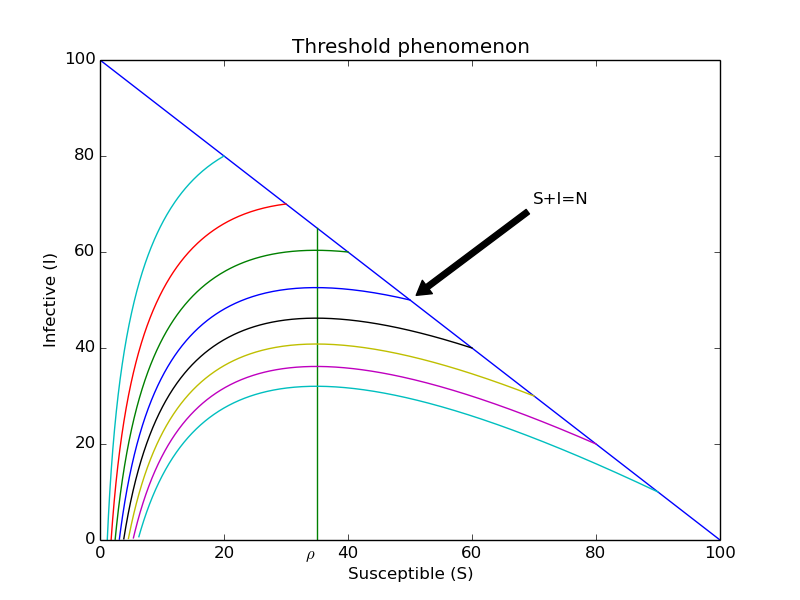
\includegraphics[width=0.9\linewidth]{plots/threshold_phenomenon.png}}
  \caption{
  \label{fig:threshold_phenomenon} Simulations of the SIR model (\ref{eq:SIR_model}) with start positions along the blue line is preformed. $I$ increases until $S$ is equal to the threshold value $\rho$, which is sat to 35. Then $I$ is reduced to 0. In the simulations where $S_0 < \rho$, no epidemic situation is achieved.
  }
\end{figure}
%\clearpage % flush figures fig:threshold_phenomenon


The simulation shows that $I$ is based on the relation between $S$ and $\rho$. This can be described with a reproduction rate,
\begin{equation}
R_0 = \frac{rS_0}{a}
\end{equation}
If $R_0 > 1$ it will cause an epidemic reaction. This parameter is crucial in the understanding of the work with the disease. To be able to keep $R_0 < 1$ will prevent a dispersion. An effective way to get control is with global vaccination programs. Smallpox is an example on a disease that nearly has been eradicated around the world. This is due to a reduction of \emph{Susceptible}. But there is always a small chance for side effects when using vaccination. And therefore some people choose to skip it. This is quite critical for the fight of total eradication. Not only is it a big risk for the specific person, but it also increase the number of \emph{Susceptible}. An epidemic situation can quickly grow again if the reproduction rate reaches the threshold.
\\
\\
Some analytical studies can be done on the simple model(\ref{eq:SIR_model}).
\begin{equation} 
\frac{dI}{dS} = -\frac{(rS-a)I}{rSI} = -1 + \frac{\rho}{S},\hspace{8mm}\rho=\frac{a}{r}, (I\neq0).
\end{equation}
The singularities will all lie on the I=0 axis. This equation can be integrated and will then give phase plane trajectories in the (I,S) plane. This can be seen in the figure(\ref{fig:threshold_phenomenon}).
\begin{equation} \label{eq:constant}
I+S-\rho \ln S = \textrm{constant} = I_0 + S_0 - \rho \ln S_0
\end{equation}
An observation is that all initial values satisfy $I_0+S_0=N$ since $R(0) = 0$. This will change when $t>0$. If a disease appears it would be important to know the severity of the disease and the chance of developing to an epidemic disease. Therefore the maximum value $\Imax$ which occurs when $S=\rho$ is crucial to know. At this point, $\frac{dI}{dt}=0$. This can be found by using (\ref{eq:constant})
\begin{align} 
I+S-\rho \ln S =& I_0 + S_0 - \rho \ln S_0 \nonumber \\
\Imax+\rho-\rho \ln \rho =& I_0 + S_0 - \rho \ln S_0\nonumber \\
\Imax=&- \rho+\rho \ln \rho + I_0 + S_0 - \rho \ln S_0\nonumber \\
\Imax=&N - \rho + \rho \ln\frac{\rho}{S_0} \label{eq:max_I}
\end{align}
The different trajectories in the figure (\ref{fig:threshold_phenomenon}) shows the difference between $S_0 > \rho$ and $S_0< \rho$. An increasing of \emph{Infective} will occur in the cases where $S_0$ is higher. While a decreasing will happen when $S_0$ is lower. An example can be shown. The $\rho$ in the simulation in figure(\ref{fig:threshold_phenomenon} is sat to 35. While $N=100$ for all trajectories. A calculation can be done on the lowest trajectory which has the initial conditions $S_0= 90$ and $I_0= 10$
\begin{align*}
\Imax =& N-\rho + \rho \ln \frac{\rho}{S_0}\\
\Imax =& 100-35 + 35 \ln \frac{35}{90}\\
\Imax =& 31.94
\end{align*}
This situation causes an epidemic situation since $\Imax$ is quite much higher than the initial condition I_0. The figure(\ref{fig:threshold_phenomenon}) shows that the trajectory of this function starts decreasing after this point. In the two upper trajectories where $S_0< \rho$, the \emph{Infective} starts decreasing from initial condition. \emph{Infective} will move towards zero as $t\rightarrow \infty$.
\\
\\
The \emph{Susceptible} will always have a decreasing solution since $\frac{dS}{dt}<0$ when $S\neq0$ and $I\neq0$. From the ODE system(\ref{eq:SIR_model}) some integration can be done,
\begin{equation} \label{eq:S_infty}
	\begin{aligned}
	\frac{dS}{dR} =& -\frac{S}{\rho}\\
	S =& S_0e^{-R/\rho} 
	\end{aligned}
\end{equation}
Then the following term is then true,
\begin{equation} 
S = S_0e^{-R/\rho} \geq S_0e^{-N/\rho} > 0
\end{equation}
As $t\rightarrow \infty$ the total number of \emph{Susceptible} will be in the range $0< S(\infty)\leq N$. This range can be reduced even more by knowing that $I$ will increase as long as $S> \rho$. The number of \emph{Susceptible} will be in the range $0< S(\infty)\leq \rho$. Since $I$ will be zero when the time goes towards infinity the \emph{Removed} class can be described $R(\infty)= N -S(\infty)$. Now this can be insert in eq(\ref{eq:S_infty}), which gives,
\begin{equation}
S(\infty) = S_0 \exp\left(-\frac{N-S(\infty)}{\rho}\right)
\end{equation}
$S(\infty)$ can be found as the positive root in the transcendental equation. This can be used to find the total number of people who catch the disease.
\begin{equation} \label{eq:total_I}
I_{total} = I_0 + S_0 -S(\infty)
\end{equation}
This analysis is based on the implication that the disease dies out because the \emph{Infective} class goes towards zero, and not because of the lack of \emph{Susceptible}. This will affect the number of \emph{Susceptible} that can be infected. This removal rate will also varies with respect to different parameters as population density, incubation time and the length of the period of sickness. The two equations (\ref{eq:max_I}) and (\ref{eq:total_I}) gives an understanding of the maximum and total number of \emph{Infective}, but the methods demand the exact number of $\rho,I_0,S_0$ and $S$, which is quite hard to get exactly in a real situation. The challenging thing is often to know how many that are infected at each time. The number of \emph{Removed} is often the easiest group to control.. This group is assisted with medical help. So to model a realistic situation, the number of \emph{Removed} as a function of time $dR/dt$ is a realistic model. Here the equations from (\ref{eq:SIR_model}) ,(\ref{eq:SIR_N}) and (\ref{eq:S_infty}) can be used.
\begin{equation} \label{eq:dR_normal}
	\begin{aligned} 
	\frac{dR}{dt} =& aI\\
	=& a(N-R-S)\\
	=& a(N-R-S_0e^{-R/\rho}), R(0)=0,
	\end{aligned}
\end{equation}
This solution demands several parameters as $a$, $r$, $S_0$ and $N$ to solve this numerically. It is normal to adjust the parameters after the epidemic situation to get the best result as possible. But if the epidemic is not to large, $R/\rho$ will be quite small, at least under 1. Then another model from Kermack and McKendrick(1927) can be used. J.D Murray does a deeper study of this in his book \cite[p.~324]{murray2002mathematical}.~This chapter will look at an example from a boarding school in England and do some studies on the change in $\rho$.  

\subsection{Epidemic in an English Boarding School 1978}
The British medical journal had in 1978 a report from a boarding school in England. One of the boys had brought with him a disease back to the school. Since this was a boarding school, they were totally isolated from others and had a closed system to model \cite[p.~325]{murray2002mathematical}.~The simulation can be seen in figure(\ref{fig:english_boarding})  


\begin{figure}[ht]
  \centerline{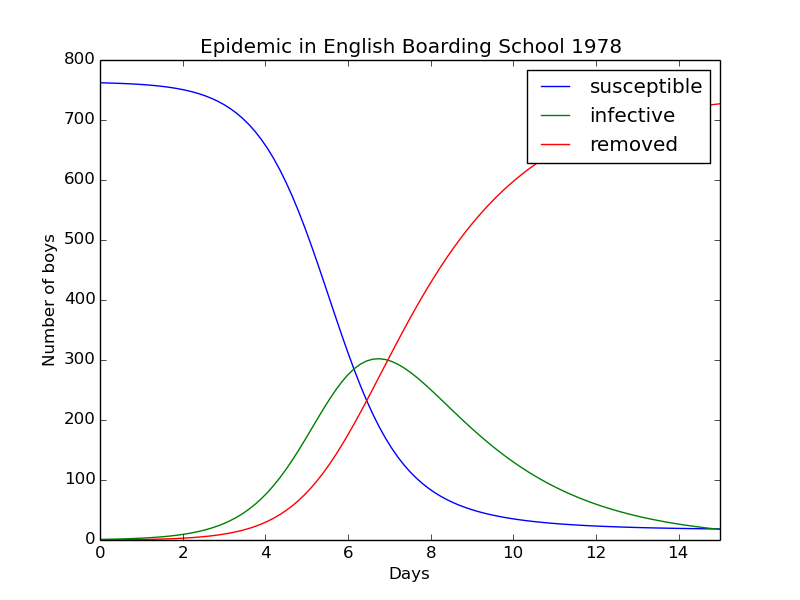
\includegraphics[width=0.9\linewidth]{plots/English_boarding_school.png}}
  \caption{
  \label{fig:english_boarding} An English boarding school is modeled for 14 days with the following parameters: $N=763$, $S_0=762$, $I_0=1$, $R_0=0$, $\rho=202$ and $r=2.18 x 10^{-3}$. An increasing of \emph{Infective} can be seen since $S_0 > \rho$.
  }
\end{figure}
%\clearpage % flush figures fig:english_boarding


The parameter value $\rho$ has a major impact on the result. The epidemic disease could turn out quite different than in the situation in figure(\ref{fig:english_boarding}) by variations in $a$ and $r$. Figure(\ref{fig:rho_changes}) consist of some examples where $\rho$ varies from 50 up to 400.


\begin{figure}[ht]
  \centerline{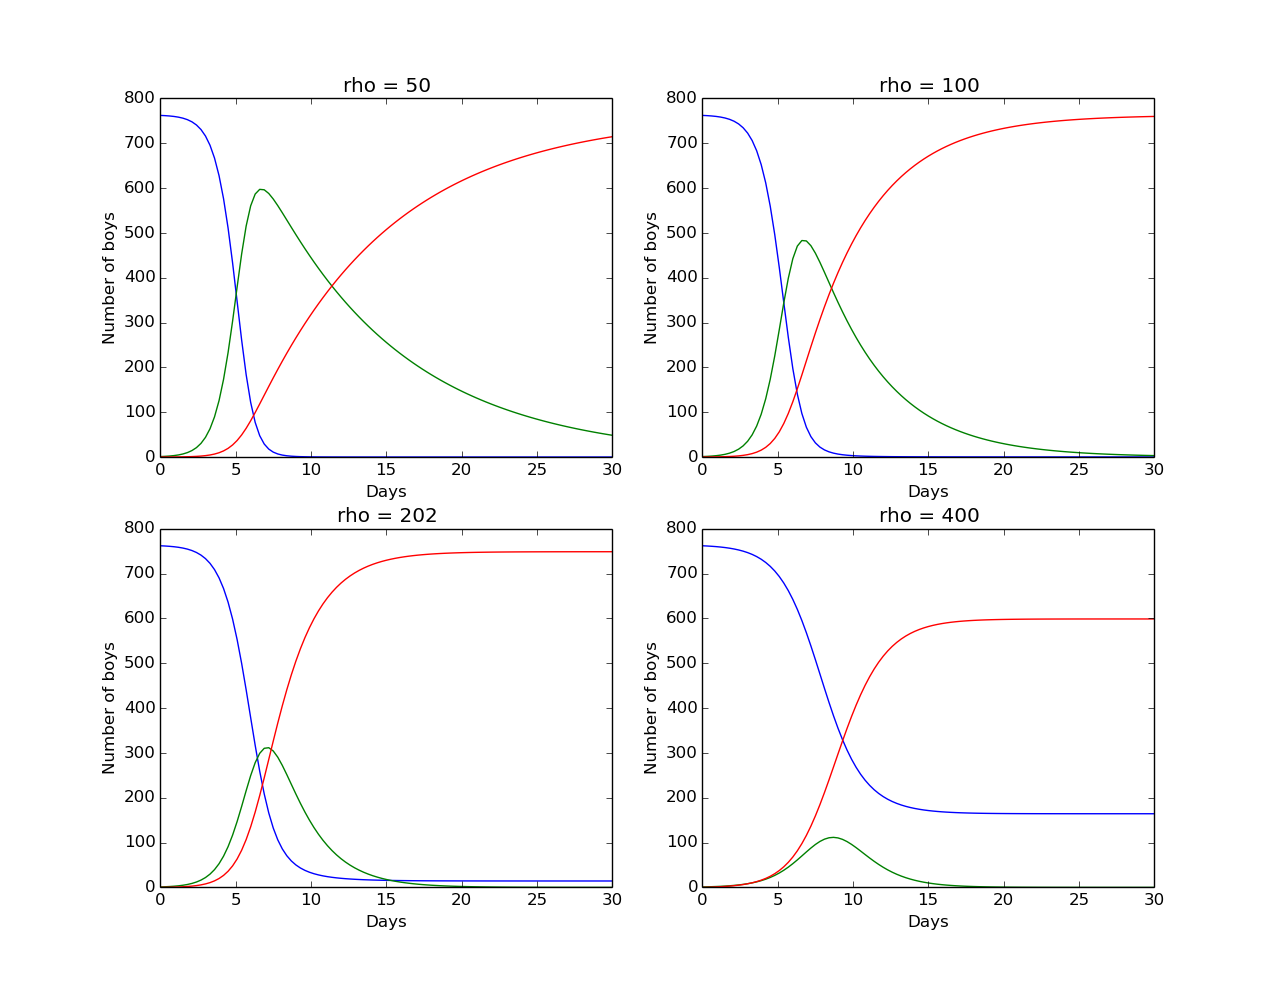
\includegraphics[width=0.9\linewidth]{plots/English_boarding_school_changes.png}}
  \caption{
  \label{fig:rho_changes} A small $\rho$ gives an aggressive disease, since $I$ will increase until $S= \rho$. In the first plot where $\rho=50$, the \emph{Infective} will increase until the number of \emph{Susceptible} falls down to 50. This will result in a majority of infected students. In the last plot where $\rho=400$, the total number of \emph{Susceptible} stays around 170 students and will go towards a steady number as $I(\infty)=0$.
  }
\end{figure}
%\clearpage % flush figures fig:rho_changes


\section{Zombification}
One of the worst epidemics that can affect the human population is a zombie attack. This will have a huge impact on the way humans live today. Several movies and series has illustrated this type of situation, but it is time that the scientists also take this threat seriously. There have been written a couple of papers about this. Munz et. al\cite{munz2009zombies} used the SEIR model to simulate an possible upcoming zombiefication, where the latent class($E$), is replaced with an \emph{Infected} class($I$) and the \emph{Infected} class($I$) is replaced with a \emph{Zombie} class($Z$). Here it is important to know that the \emph{Infected} class in the $SIZR$ is not the same as in the $SEIR$ model presented earlier. The following model was used,

\begin{align*}
\frac{dS}{dt} =& \Sigma -\beta SZ - \delta S \\
\frac{dI}{dt} =& \beta SZ - \varrho I - \delta I\\
\frac{dZ}{dt} =& \varrho I + \zeta R - \alpha SZ\\
\frac{dR}{dt} =& \delta S + \delta I + \alpha SZ - \zeta R
\end{align*}

This is a bit more complicated than the standard $SEIR$ model. A presentation of the parameters;
\begin{itemize}
\item $\Sigma$ describes the birthrate for new \emph{Susceptible}. $\frac{dS}{dt}$ is now able to be positive. This is now not a closed system. 

\item $\beta SZ$ describes the numbers of \emph{Susceptible} that become \emph{Infected} , based on interactions between zombies and humans. Similar as the case for $rSI$ in the SIR model. 

\item $\delta$ describes the number of naturals deaths among the group. This is used in the \emph{Susceptible} and the \emph{Infected} group

\item $\varrho I$ describes the probability for an infected human to wake up as a zombie.

\item $\zeta R$ controls the number of \emph{Removed} that arises as \emph{Zombie}. 

\item $\alpha SZ$ describes the number of zombies killed by humans in the zombie attacks. 
\end{itemize}

\noindent
\\
\\
This model was challenged by Langtangen, Mardal and Røtnes \cite{zombie-math} now referred as LMR, where they developed another model. They had three objections to the model from Munz et al.~\cite{munz2009zombies}.They argue that dead zombies cannot become functioning zombies again. Therefore $\zeta$ will be zero, if not magic is introduced. They let the parameters in the model change with time, according to different phases. They argue that the behavior will change with time during a zombie attack. The parameters in the model is based on the movie \emph{The Night of The Living Dead}. This is done to reproduce its scenarios and then predict how a zombie outbreak would appear. There is also added a function $\omega(t)$, which creates a massive attack from the humans. This is controlled by a time variable and give the \emph{Susceptible} a chance to fight back. The system can be seen in eq(\ref{eq:LMR_model}):
\begin{equation} \label{eq:LMR_model}
	\begin{aligned} 
	\frac{dS}{dt} =& \Sigma -\beta SZ - \delta_SS \\
	\frac{dI}{dt} =& \beta SZ - \varrho I - \delta_II\\
	\frac{dZ}{dt} =& \varrho I- (\alpha+\omega(t))SZ + \zeta R\\
	\frac{dR}{dt} =& \delta_SS +\delta_II -\zeta R + (\alpha+\omega(t))SZ 
	\end{aligned}
\end{equation}
The main change here is the $\omega(t)$ introduced above. This is a Gaussian curve and can be seen in eq(\ref{eq:omega}).
\begin{equation} \label{eq:omega}
\omega(t) = a \sum^m_{i=0}\exp\left(\frac{1}{2}\left(\frac{t-T_i}{\sigma}\right)^2\right)
\end{equation}
$\omega(t)$ controls the attacks from the \emph{Susceptible}, which will be fired at predefined time steps. These are controlled by the three parameters. 
\begin{itemize}
\item $a$ here works as a similar parameter as $\alpha$, but will only be activated when the \emph{Susceptible} group is organized and ready to attack. 

\item $T$ contains a list of numbers, which controls the time when the attacks will occur.

\item $\sigma$ controls the length of the attack. 
\end{itemize}

\noindent
This function will be modeled later when it is used in the Section~\ref{section:counter_attack}
\\
\\
\subsection{Threshold phenomenon}
This section is connected to the section \emph{Threshold phenomenon} earlier in this paper. It is under construction and will be removed if it is not relevant. Some notes for the writer:
\begin{itemize}
\item \cite[p.~22]{zombie-math}

\item \cite[p.~136-142]{munz2009zombies}

\item perspectives on the basic reproductive ratio

\item Reproduction numbers and sub-threshold endemic equilibria for compartmental models of disease transmission
\end{itemize}

\noindent
\subsection{Parameters used in the model}
The parameter values are an essential factor while modelling a zombie attack. Data from the movie \emph{The Night of The Living Dead} was used as basis for the parameters in the ODE system from LMR \cite{zombie-math}. This thesis has study the TV series \emph{Walking dead} in detail \cite{walking_dead}. The data will be based on the first five episodes and are constructed by watching the episodes carefully. The three phases in a zombie attack will be based on the form used in the paper from LMR, but with an extending version in the \emph{Counter attack phase} .

\paragraph{The initial phase.}
the disease is yet not known in this phase and humans try to save the sick ones by taking them to hospitals or get some kind of treatment. Because of this ignorance related to the disease, the number of infected humans is high. This phase is often quite short and humans soon start to realise that the risk of getting infected by saving other is really high. \emph{Walking Dead} never shows anything from this phase, but the viewer sees the damages done when the main character sheriff Rick Grimes wakes up at the local hospital. What he wakes up to is the major damage caused in the initial phase, while the society has moved to the hysterical phase.
\\
\\
To determine the values for each group in each phase, the length of Ricks coma is essential. There are several factors that gives an indication of the time aspect. When Rick wakes up at the hospital he has grown a smooth beard of about 1 cm. This would correspond to 1 month in average for an European origin. He also has some flowers which has dried out, these also give the impression that there has been some weeks. The hospital is running on its emergency generator. This would probably not last for many days with a fully operational hospital, but the hospital is as well as shut down when Rick wakes up and can give the emergency generator a longer lifetime. Dr.~Edwin Jenner gives the viewer some information in episode 5 where tells the videolog that it was 63 days since the epidemic started spreading. By studying the first five episodes in detail, the series gives a sense that the time aspect has not been in focus. Therefore the different phases are constructed from the information that has been given. Rick Grimes has probably been in coma for a month and what he meets the first days will be the basis. The total amount of objects in the model will be based on the number of humans, dead and zombies seen in the first five episodes. 
\begin{itemize}
 \item The number of humans has been estimated to \textbf{62}. 20 living in the camp with Rick, 40 humans in the old nursing home and the father and son in episode 1. 

 \item The number of dead is estimated to \textbf{200}. This is based on the amount of dead outside the hospital where Rick woke up. 

 \item The number of zombies are assume to be \textbf{360}. These are based on the 30 outside the house of Morgan Jones and his son Duane, 300 zombies in the city Atlanta and 30 zombies attacking the camp. 
\end{itemize}

\noindent
The total number will be \textbf{622} and the time aspect aroud a month, which means that these numbers are for the hysterical phase.Over the three first days when Rick is awake 1 human and about 20 zombies are killed by each other. This can be used to calculate the final number in the initial phase by calulating backwards. To do this calculation easier, a month is assumed to be 30 days and 27 days earlier become 9 similar periods  with the same amount of deaths. This results in 180 zombies and 9 humans killed in this period. The final number for the initial phase can then be set to 71 humans, 540 zombies/infected and 20 dead. This is the same number as for the initial values for the hysterical phase, since the phases are connected.
\\
\\
Another question to discuss is the incubation time. Here there are two examples that can be used. The first transformation from human to zombie happens for the character Amy, who was bit in the arm by a zombie. The transformation happens in about 12 hours. The other example is character Jim which has a slower transformation. This last for about two days before the rest of the group leave him alongside the road on their way to CDC(Center for Disease Control). An estimate of the incubation time can be set to 24 hours based on these two transformations.
\\
\\
Now the ODE system (\ref{eq:LMR_model})can be used to model the initial phase. The expected results are $S_0 = 621$ and $Z_0 = 1$ while the two other groups are set to zero. The value of $\beta$ can be found with the expression $\beta \Delta t S Z$ from the first ODE equation. After three days about 90 percent of the humans are killed.
\begin{equation}
	\begin{aligned}
	\beta\Delta t S Z &= 0.1 S\\
	3\beta   &= 0.1 \\
	\beta &= 0.33 \\
	\end{aligned}
\end{equation}
The probability for a human being infected will be sat to $\beta \approx 0.3$. The natural death rate is sat to $\delta_S = 2.2*10^{-5}$ based on numbers from CDC \cite{CBC_deaths_2011}. It is quite hard to find similar realistic data for infected humans, so $\delta_I = \delta_S$. The number of births is sat to $\Sigma = 3.45*10^{-5}$. This is based on data from CDC from 2012 \cite{CBC_births_2012}. Since this is data for the initial phase, zombies are seen as infeteced humans that can be saved. Therefore $\alpha = 0$. And the two last parameters are also zero, $a = \zeta = 0$. The initial phase is modeled in figure(\ref{fig:initial_phase_1}):


\begin{figure}[ht]
  \centerline{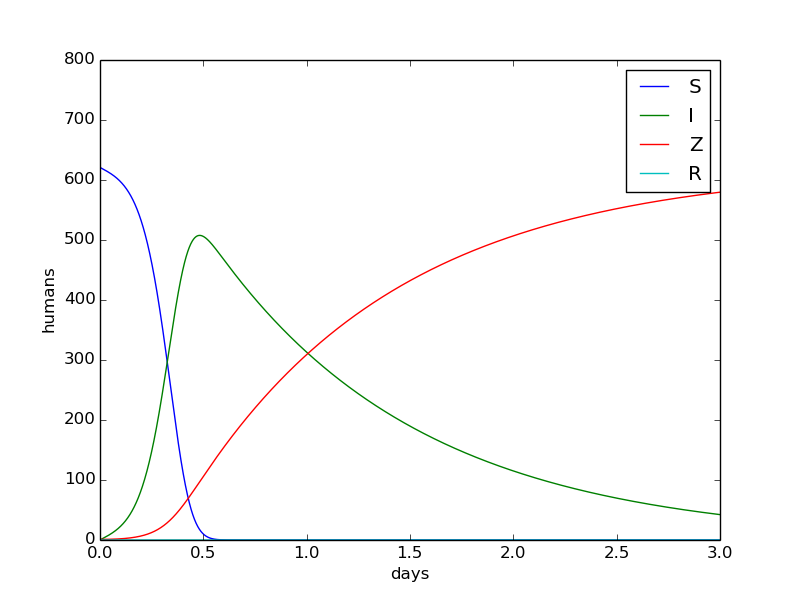
\includegraphics[width=0.9\linewidth]{plots/WD_zombie_initial_1.png}}
  \caption{
  \label{fig:initial_phase_1} Initial phase for \emph{Walking Dead}. $\beta=0.3$, $\varrho=1$ and $\alpha=0$ leads to eradication.
  }
\end{figure}
%\clearpage % flush figures fig:initial_phase_1


The result from figure(\ref{fig:initial_phase_1}) shows that the human population is eradicated in about a half day. This is not the case, and some adjustments need to be done. There are three parameters that are interesting to study. The first one is $\beta$, which describes how many humans that get infected in a human-zombie collision. Second one is $\varrho$. This parameter controls the incubation time. The last parameter that can affect the number in each group is $\alpha$. This describe the number of zombies killed in a human-zombie collision. These variables are plotted separately and combined in figure(\ref{fig:initial_parameters}). The idea here is to produce results that fulfill the final number for the classes \emph{Susceptible} and \emph{Removed} , which is 71 and 20. The blue dot in each plot is describe this value. A rough estimate has been done for each parameter before using it. This is why they all lie in different regions than the parameter value in figure(\ref{fig:initial_phase_1})



\begin{figure}[ht]
  \centerline{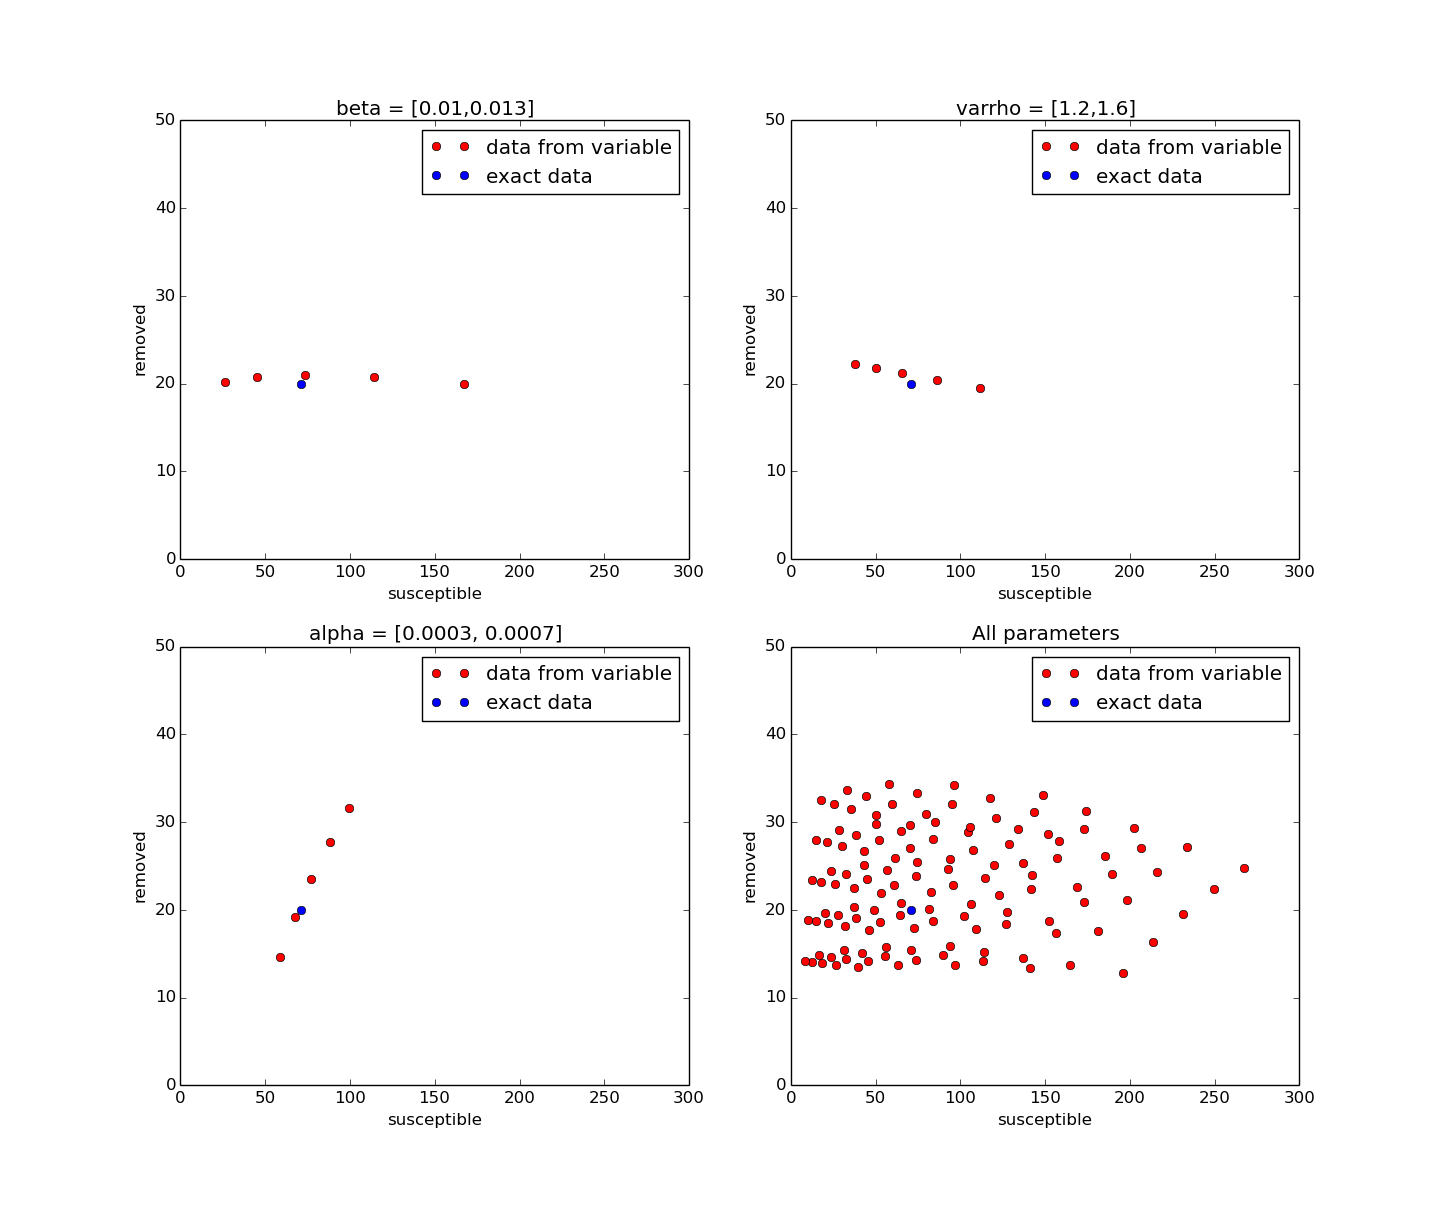
\includegraphics[width=0.9\linewidth]{plots/check_parameters.png}}
  \caption{
  \label{fig:initial_parameters} These plots give an important knowledge in the effect of varying the parameters. $\beta$ and $\varrho$ mainly affect the number of \emph{Susceptible} while $\alpha$ affect them both.
  }
\end{figure}
%\clearpage % flush figures fig:initial_parameters


By choosing $\beta = 0.01155$, $\varrho=1.37$ and $\alpha=0.00044$, the following plot can be seen in figure(\ref{fig:initial_phase_2}):  


\begin{figure}[ht]
  \centerline{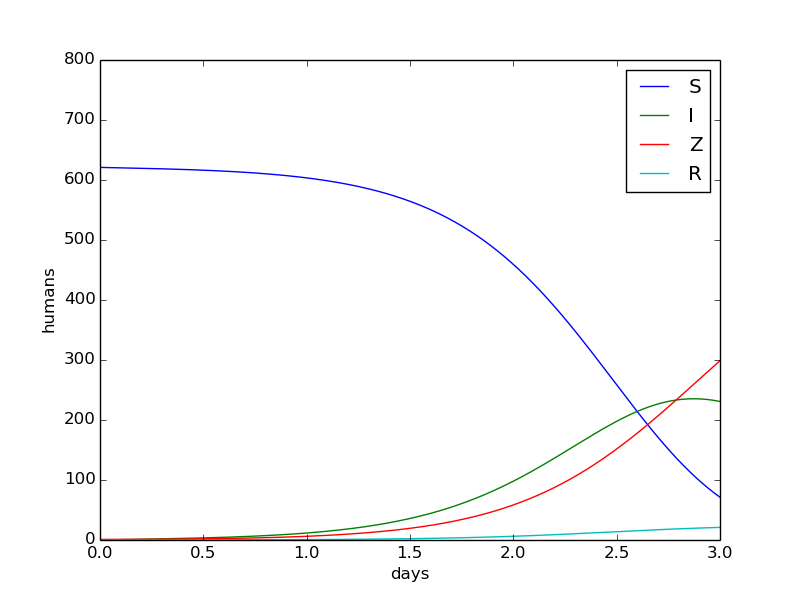
\includegraphics[width=0.9\linewidth]{plots/WD_zombie_initial_2.png}}
  \caption{
  \label{fig:initial_phase_2} The final values are $S_n=71.3,I_n=230.8,Z_n=298.9$ and $R_n=21$, which is quite close to the result from the movie.
  }
\end{figure}
%\clearpage % flush figures fig:initial_phase_2


It is possible to argue for the changes done in figure(\ref{fig:initial_phase_2}). Increasing $\varrho$ to 1.37 reduces the incubation time. Now the average time will be about 17.5 hours which is quite realistic. The probability $\beta$ is quite sensitive and has a major effect only by small variations. This is due to the term that it is a part of $\Delta t SZ \beta$. A couple of examples demonstrate this. One hour can be estimated by setting $\Delta t$ = 1/24$. When using the initial values for the classes $S$ and $Z$ and $\beta=0.01155$ from figure(\ref{fig:initial_phase_2}), the number of infected in the first hour will be $(1/24)*721*1*0.01155=0.34$. About  one-third of a human in the first hour seems as a slow and not very aggressive disease. But when the number of \emph{Zombies} slowly increase, the number of infected will be affected. By looking at the hour when the values are equal between humans and zombies, about 200 in each group, the number of infected will be 19.25 per hour. This result in about 10 percent of the humans. By changing $\beta$ to the value from figure(\ref{fig:initial_phase_1}), the number of infected will be 500 per hour and it is quite easy to see that this will lead to eradication in a short amount of time. The last parameter $\alpha$ controls the number of zombies that dies in collisions between zombies and humans. While humans still think that the infected can be saved, it is still a chance that the result from a collision can end with a murder. These results can therefore be seen as realistic values.

\paragraph{The hysterical phase.}
Now the humans start to avoid the infected and some try to fight them. The humans often gather in groups and try to find safe spots away from the zombies. Important emergency as weapons and food are their main priority. Barricades are built and the guarding is strict. When Rick Grimes wakes up, the hospital is abandoned and the halls are filled up with dead people. Quite fast he understand that he needs to reach safety and after a couple of days he ends up in a camp outside Atlanta city. A couple of elementary changes has happen with the interaction between humans and infected/zombies. In the initial phase, the humans tried to help the infected humans. This resulted in a high percent of infected. While they now understand this risk and keep distance to those who are infected. This will give $\beta$ a lower value. The morality for a zombie kill has dramatically changed. While this was seen as no opinion in the initial phase, this is now okay. The humans have started to treat zombies and infected as enemies instead of sick allies. This result in a higher death rate among the zombies, which is described by $\alpha$. 
\\
\\
The hysterical model can be constructed based on the data found in the initial phase. 


\begin{quote}
\begin{tabular}{ccc}
\hline
\multicolumn{1}{c}{ hysterical phase } & \multicolumn{1}{c}{ initial values } & \multicolumn{1}{c}{ final values } \\
\hline
S                & 71.3             & 62               \\
I                & 230.8            & -                \\
Z                & 298.9            & 360              \\
R                & 21               & 200              \\
\hline
\end{tabular}
\end{quote}

\noindent
Here infected and zombies are counted as one group in the final values, since it is difficult to separate these grops in the series. The time aspect will be modeled for 30 days, which result in ten times longer simulation. Since the final results are known here, a similar adjustment of the parameters can be done. The range of the parameter values have been found by some test simulations.In figure(\ref{fig:hysterical_variations}) the values of $\beta$,$\varrho$ and $\alpha$ has been simulated with different values. 


\begin{figure}[ht]
  \centerline{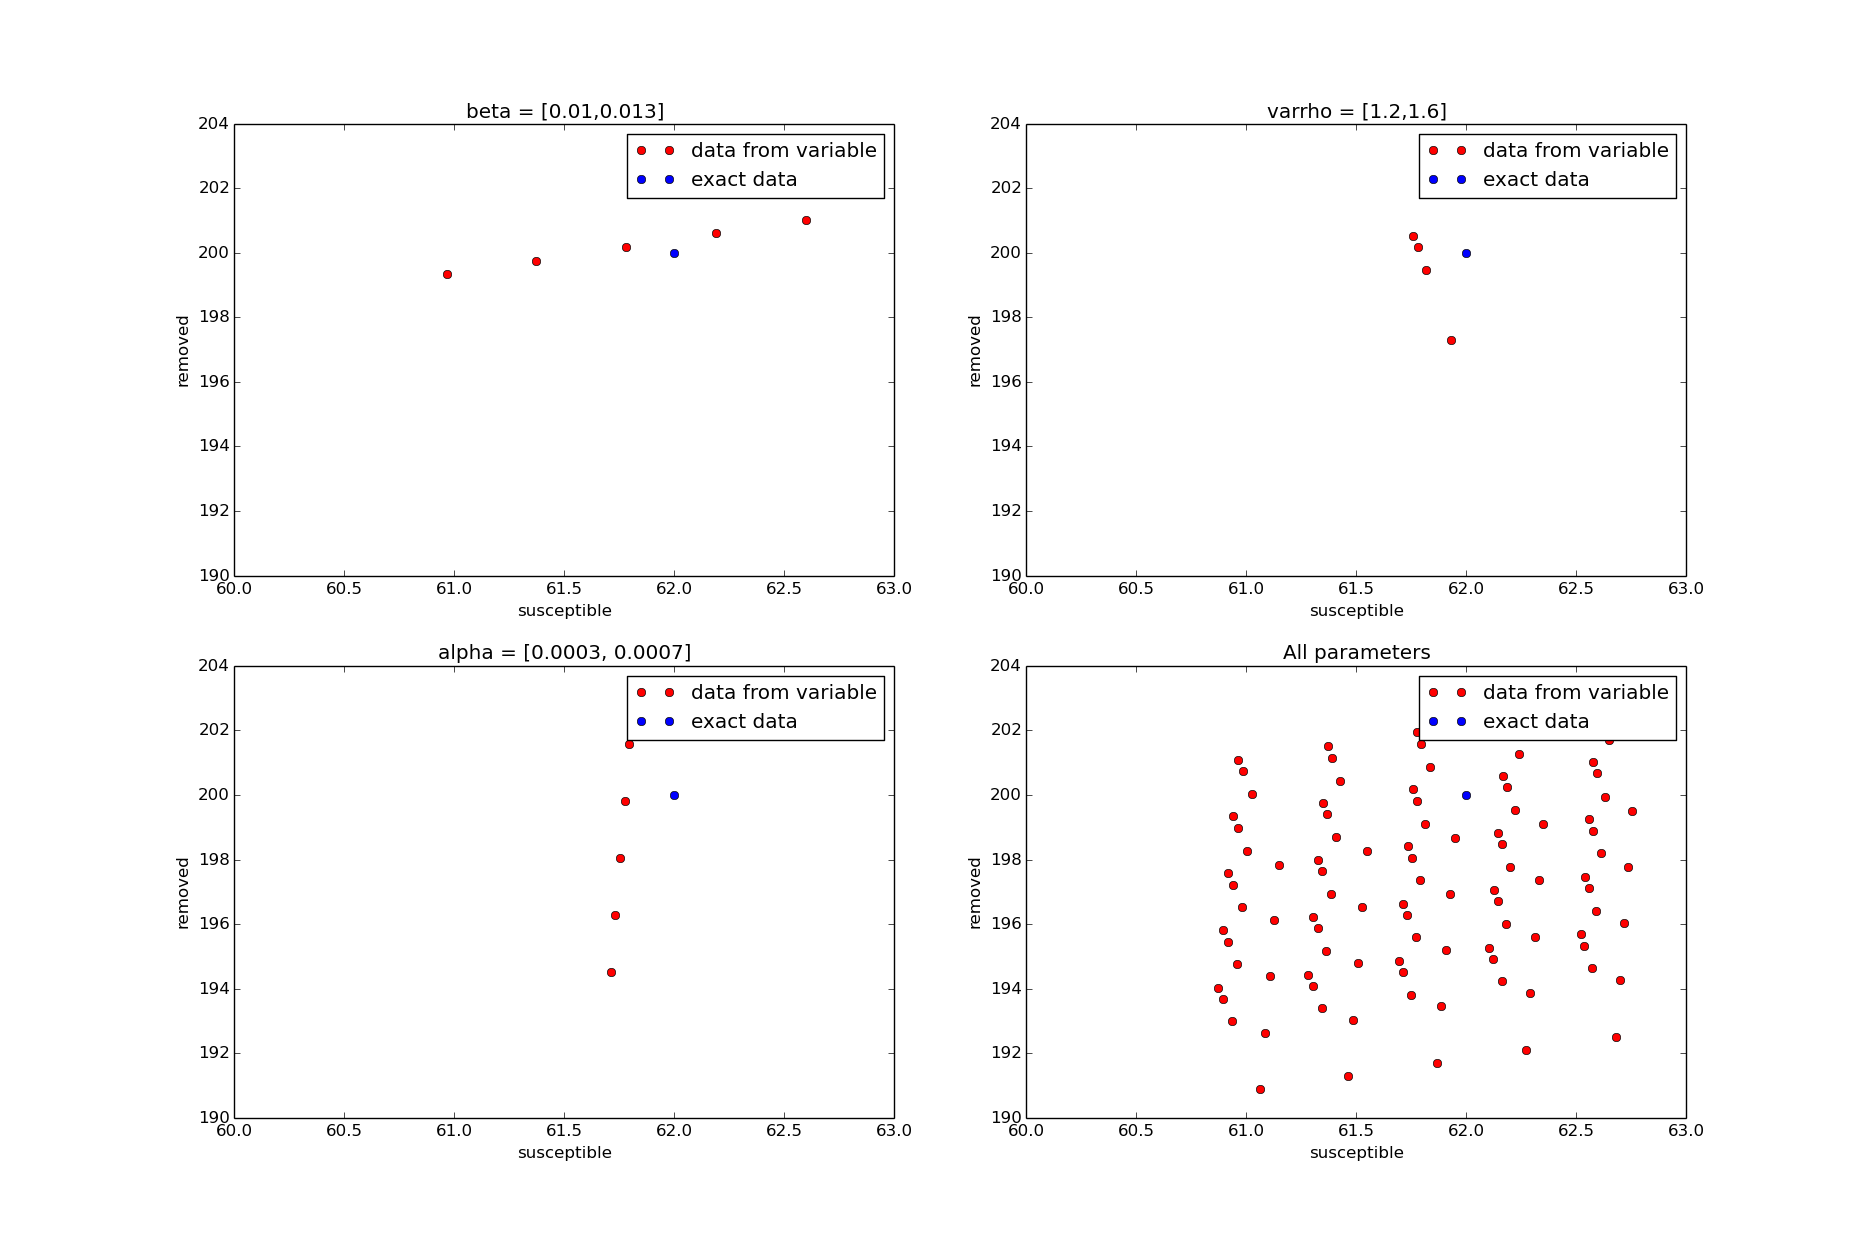
\includegraphics[width=0.9\linewidth]{plots/check_parameters_hysterical_2.png}}
  \caption{
  \label{fig:hysterical_variations} Variation in three different parameters in the hysterical phase. The last subplot consist of the combination of all. $\beta=[1*10^{-5},1.2*10^{-5}]$, $\varrho=[1,2]$ and $\alpha=[2*10^{-4},2.2*10^{-4}]$
  }
\end{figure}
%\clearpage % flush figures fig:hysterical_variations


Figure(\ref{fig:hysterical_variations}) gives insight in how the variations in parameters affect the final result. By decreasing $\beta$, it will essentially increase the number of \emph{Susceptible} that will survive. But it will also increase the number of deaths. This may at first glance seems quite strange. Should not the number of deaths decrease when the number of surviving humans increase? This can be explained with the idea that was shown for $\beta$ in the initial phase. Since $\beta SZ$ gets smaller when $\beta$ get smaller, the combination of $SZ$ will stay higher for a longer time . This again affect $\alpha SZ$, which regulates the number of killed zombies. The larger this combination is, the more zombies will die. 
\\
\\
By increasing $\alpha$, the number of \emph{Removed} also increase. But similar to the increasing of the \emph{Removed} it also has a slight increase on the number of \emph{Susceptible}. Here the argument for $\beta$ above can be reversed. Since a higher $\alpha$ leads to a higher death rate among the zombies, the combination $SZ$ will be smaller which make $\beta SZ$ smaller.
\\
\\
The last parameter, $\varrho$, has nearly no effect. The red dots show a small decreasing of \emph{Removed} and increasing of \emph{Susceptible}  when $\varrho$ is increased. This parameter varies most, but has least impact. This can be explained with the long time aspect and the low number of infected compared to the number of zombies. Since the number of zombies are that much higher, the transformation length from infected to zombie is almost negligible.  


\begin{figure}[ht]
  \centerline{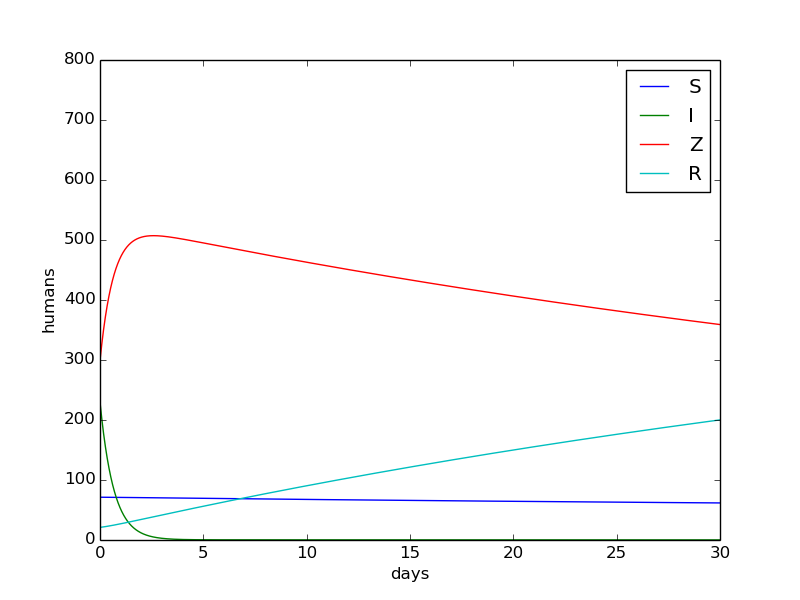
\includegraphics[width=0.9\linewidth]{plots/WD_zombie_hysterical_1.png}}
  \caption{
  \label{fig:hysterical_1} Hysterical phase with parameter values $\beta = 0.000011$, $\varrho = 1.5$ and $\alpha = 0.000208$.
  }
\end{figure}
%\clearpage % flush figures fig:hysterical_1


Figure(\ref{fig:hysterical_1}) fulfills the result that was predicted based on the series. These final numbers correspond to the number in each group when Rick woke up at the hospital. The plot shows that the number of zombies increase quickly and reach its maximum value after a couple of days in this phase, similar the number of infected dramatically decreased. Here the humans have been able to stabilize. Since the clashes between humans and zombies are dramatically decreased, there are nearly no humans that get infected. And in the cases where humans has to face zombies, the kill rate has increased. The increase of \emph{Removed} is close to proportional to the decrease of \emph{Zombies}, which means that there are mostly zombies that dies.

\paragraph{The counter attack.}
\label{section:counter_attack}
This counter attack is more complicated to model since this phase appear simultaneously as the hysterical phase in \emph{Walking Dead}. The group of human are trying to avoid the zombies, but when the zombies get to close, the humans need to fight back. These situations are caused by a high density of zombies in some areas. This force the zombies to spread. In \emph{Walking dead} the counter attack appears when a group of 30 zombies reach the camp. This trigger a fight where all the zombies are killed and 4 of the humans got bitten. This shows that a counter attack from the humans causes a lot of damage. The time aspect is sat to 6 hours.  
\\
\\
Now the function $\omega(t)$ will be used. This can be seen in figure(\ref{fig:omega_function}):


\begin{figure}[ht]
  \centerline{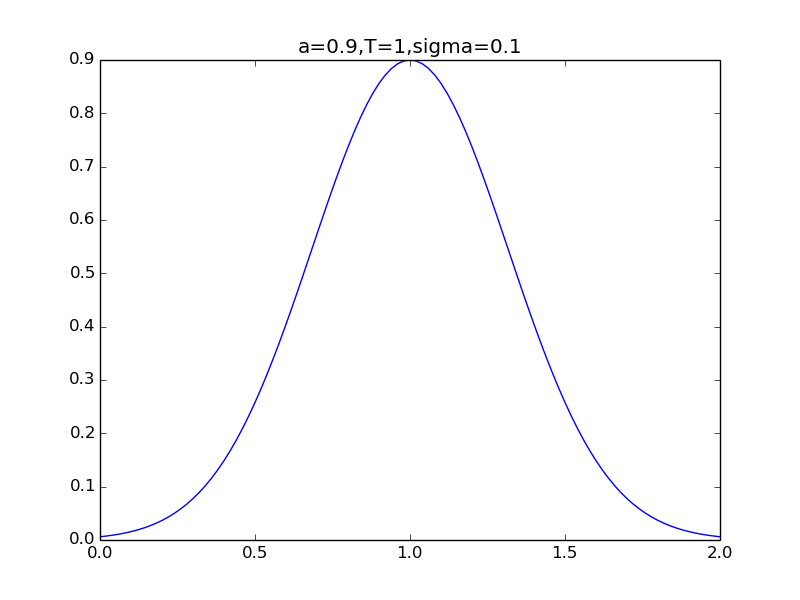
\includegraphics[width=0.9\linewidth]{plots/omega_function.png}}
  \caption{
  \label{fig:omega_function} $\omega (t)$ is a Gaussian function where $a$ controls the maximum value, $T$ controls the time for maximum value and $\sigma$ controls the length of the attack.
  }
\end{figure}
%\clearpage % flush figures fig:omega_function


To get some start values, $SZ\omega(t)=30$ can be used. Where $\omega(t)$ is the area under the function. By inserting the final values from hysterical phase for $S$ and $Z$, the area shall be $\omega (t)=1.34*10^{-3}$. By using $a= 0.00103$ and $\sigma = 0.005$ in $\omega(t)$, this result can be reproduced. The counter attack is sat to appear during the last part of the day [0.75,1]. The value of T is then sat to $T=[0.875].


\begin{figure}[ht]
  \centerline{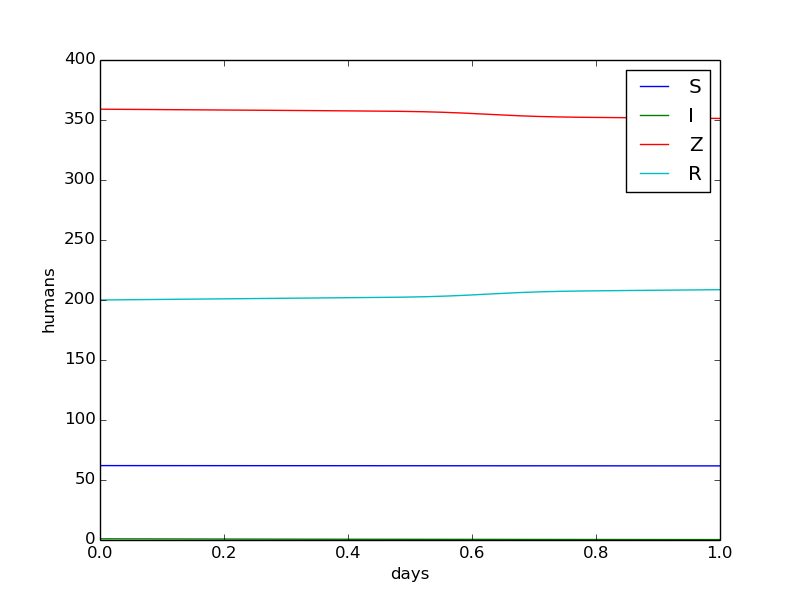
\includegraphics[width=0.9\linewidth]{plots/WD_zombie_counter_1.png}}
  \caption{
  The counter attack. 8-9 zombies are killed and all humans survive
  }
\end{figure}
%\clearpage % flush figures 


This simulation in figure(\ref{fig:zombie_counter_1}) result in some deaths,but the total number should be higher. Another problem is that no human died under this battle. The ODE model (ret{eq:LMR_model}) from \cite{zombie-math} is based on \emph{The Night of the Living Dead}, where the amount of humans who are killed are close to zero. This is not the case in \emph{Walking dead}. Therefore the risk of dying is higher for human during a counter attack. This is solved by adding $\mu \omega (t) SZ$, where $\mu$ is the risk for a human to get infected compared to a zombie kill during this attack. The model (\ref{eq:LMR_model}) can then be expand,

\begin{align*} \label{eq: seland_model}
\frac{dS}{dt} =& \Sigma -(\beta+\mu \omega(t))SZ - \delta_SS \\
\frac{dI}{dt} =& (\beta+\mu \omega(t))SZ - \varrho I - \delta_II\\
\frac{dZ}{dt} =& \varrho I- (\alpha+\omega(t))SZ + \zeta R\\
\frac{dR}{dt} =& \delta_SS +\delta_II -\zeta R + (\alpha+\omega(t))SZ 
\end{align*}


\begin{figure}[ht]
  \centerline{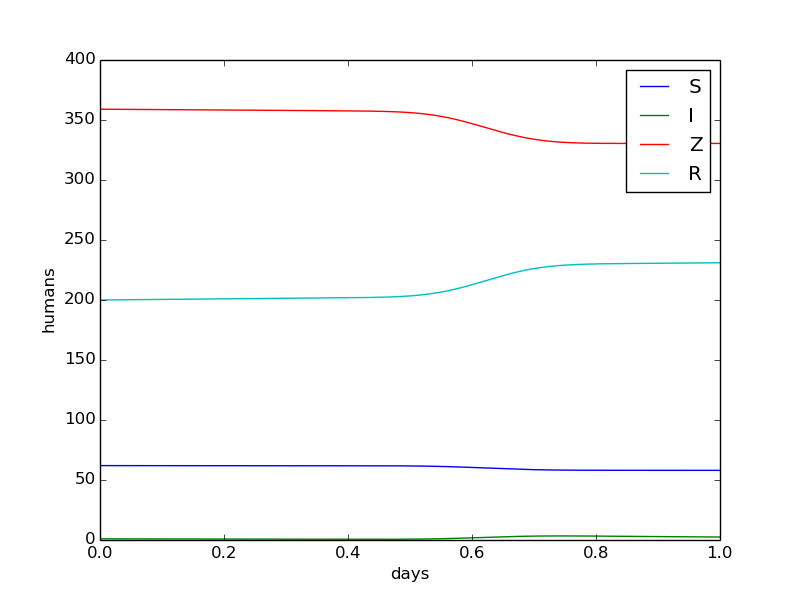
\includegraphics[width=0.9\linewidth]{plots/WD_zombie_counter_2.png}}
  \caption{
  \label{fig:zombie_counter_2} Counter attack with the new model. Parameter values are set to $a=0.0073$ and $\mu=0.14$.
  }
\end{figure}
%\clearpage % flush figures fig:zombie_counter_2


Figure(\ref{fig:zombie_counter_2}) is modeled with the initial values given when Rich woke up, explained in the initial phase. The result after this day is that the humans are reduced to 58 humans. The number of infected are increased to 2.47, which can be explained with the two characters in the series, Amy and Jim. The number of \emph{Removed} is increased to 231, and is a combination of killed zombies and humans who are attacked. By modelling this for another day, the \emph{Removed} class will increase with a couple on new deaths. 
\\
\\
An interesting situation is to check the evolution if this counter attack repeats it self for a series of time. Who will survive? An attack every other day will give the following result shown in figure(\ref{fig:counter_series})


\begin{figure}[ht]
  \centerline{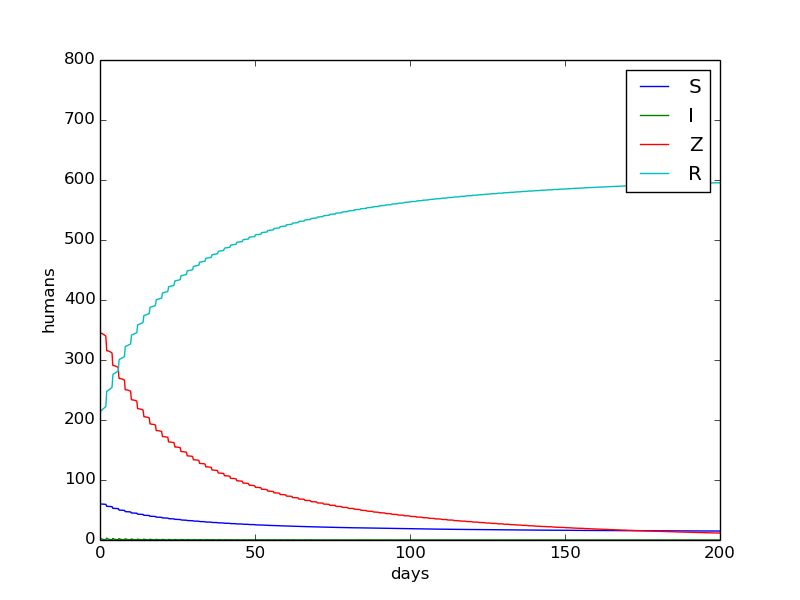
\includegraphics[width=0.9\linewidth]{plots/WD_zombie_counter_series.png}}
  \caption{
  \label{fig:counter_series} 100 counter attacks during 200 days will result in a higher population of humans.
  }
\end{figure}
%\clearpage % flush figures fig:counter_series


After 200 days there will be about 15 humans and 12 zombies left. Now the humans are able to survive since they are more efficiency in battles. There are of course several things to discuss. How will the number of battles effect the humans and zombies. Will they be tired or more efficiency? What about weapons? What would happen if the group of zombies was much larger? This paper is based on observation of the series and will therefore leave this questions to the reader. 

\paragraph{The three phases in Walking Dead.}
By adding these three phases together, the final result after the attack should be possible to match. The simulation here will be done with the parameters used in the earlier sections. This can lead to a small error since the result for the final number in each phase are given with decimals and the initial values are based on assumptions and round off numbers. The different parameter values are listed in table{ref:param_val}. 

\begin{quote}
\begin{tabular}{cccc}
\hline
\multicolumn{1}{c}{ parameter } & \multicolumn{1}{c}{ Initial phase } & \multicolumn{1}{c}{ hysterical phase } & \multicolumn{1}{c}{ counter attack } \\
\hline
$\beta$          & 0.01155          & 0.000011         & 0.00011          \\
$\varrho$        & 1.37             & 1.5              & 1.5              \\
$\alpha$         & 0.00044          & 0.000208         & 0.000208         \\
a                & 0                & 0                & 0.0073           \\
$\sigma$         & 0                & 0                & 0.005            \\
$\mu$            & 0                & 0                & 0.14             \\
\hline
\end{tabular}
\end{quote}

\noindent

The simulation is run for 34 days. The three first days are in the initial phase, the resisting days are in the hysterical phase. The counter attack is released in day 33 and last for about 6 hours. The plot is shown above   


\begin{figure}[ht]
  \centerline{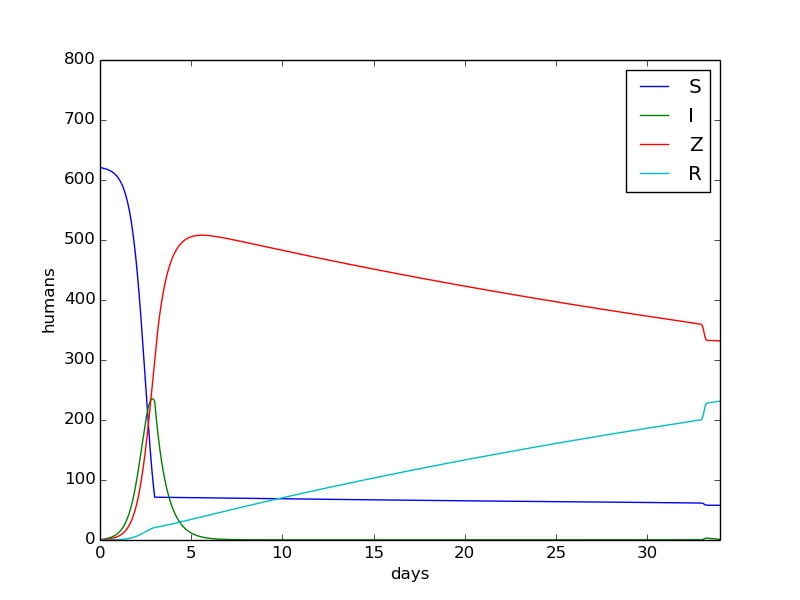
\includegraphics[width=0.9\linewidth]{plots/WD_zombie_all_phases_1.png}}
  \caption{
  Walking Dead simulated after 5 episodes. Based on the three different phases.
  }
\end{figure}
%\clearpage % flush figures 


Figure(\ref{fig:all_phases}) clearly shows that the change in parameter values affect the different phases. The different values are shown in the table(\ref{table:class_values}), where the values are given at the initial time. The last column consist of the final values after 34 days.

\begin{quote}
\begin{tabular}{ccccc}
\hline
\multicolumn{1}{c}{ --------- } & \multicolumn{1}{c}{ Initial phase } & \multicolumn{1}{c}{ hysterical phase } & \multicolumn{1}{c}{ counter attack } & \multicolumn{1}{c}{ final values } \\
\hline
S_0              & 621              & 71               & 62               & 58               \\
I_0              & 0                & 231              & 0                & 1                \\
Z_0              & 1                & 299              & 359              & 332              \\
R_0              & 0                & 21               & 202              & 231              \\
\hline
\end{tabular}
\end{quote}

\noindent

Considering the uncertainty of the parameters, this simulation gives result close to the expected result. 
\\
\\
\paragraph{Quality of this model.}
This model will be used as the basic model to compare against. The biggest advantage with this model is that it is straight forward to calculate. It it easy and quite simple to understand. This is good if the goal is to find the total number in each class measured over an area, but it gives no information about the spatial spread of the disease. This will therefore be useless in the work on describing how fast a disease can spread abroad countries and borderlines. The two next chapters will introduce more complicated models which will be compared to this ODE-system modeled here.


\bibliographystyle{plain}
\bibliography{papers}


% ------------------- end of main content ---------------


% #ifdef PREAMBLE
\printindex

\end{document}
% #endif

